\documentclass[twocolumn]{article}
\usepackage{graphicx}
\usepackage{amsmath}
\usepackage{geometry}
\geometry{margin=0.8in}
\usepackage{float}
\usepackage{placeins}
\title{The Application of Neural Ordinary Differential Equations to Experimental Predator Prey Data}
\author{Aksel Boukhalfa}
\date{July 2024}

\begin{document}
\maketitle

\begin{abstract}
The goal of this project was to investigate the integration of neural networks into systems of ordinary differential equations in order to approximate dynamics in ecological systems. This was done through the implementation of classical Lotka-Volterra models and Neural Ordinary Differential Equations (NODEs). Overall, it was found that the NODE model was capable of fitting to noisy Lotka-Volterra based training data and learning to predict trends, even extrapolating to predict oscillations. However, when applied to experimental predator-prey data, the model was overwhelmed by noise in the dataset and could not fit to the training data.
\end{abstract}

\section{Introduction}
Predator-prey population dynamics are crucial to understanding ecological systems. Classical approaches to predicting predator-prey dynamics, such as the Lotka-Volterra model, assume homogeneity among predators and prey\cite{Lotka1925, Volterra1926}. These models often fail to account for environmental factors and noise inherent in real-world data. This study aims to compare the classical Lotka-Volterra model with Neural Ordinary Differential Equations (NODEs), a novel approach that integrates neural networks into ODE systems to capture more complex dynamics.

\section{Background}

The Lotka-Volterra model, also known as the predator-prey equations, is a pair of first-order, nonlinear, differential equations frequently used to describe the dynamics of biological systems in which two species interact, one as a predator and the other as prey. Introduced independently by Alfred Lotka in 1925 and Vito Volterra in 1926, this model is foundational in the study of biological systems and mathematical biology.

\subsection{Classical Lotka-Volterra Model}
The Lotka-Volterra model describes the interdependent changes in the populations of two species over time. The equations are given by:

\[
\frac{dx}{dt} = \alpha x - \beta xy
\]

\[
\frac{dy}{dt} = \gamma xy - \delta y
\]

where \(x\) and \(y\) represent the prey and predator populations, respectively. The parameters \(\alpha, \beta, \gamma, \) and \(\delta\) are positive real numbers describing the interaction rates. Specifically:
\begin{itemize}
    \item \(\alpha\) is the growth rate of the prey in the absence of predators.
    \item \(\beta\) is the rate at which predators consume the prey.
    \item \(\gamma\) is the growth rate of the predator population per prey consumed.
    \item \(\delta\) is the natural death rate of predators in the absence of prey.
\end{itemize}

Due to its relative simplicity, the classical Lotka-Volterra model has limitations. It assumes that the environment does not change over time and that all predators and prey are functionally identical. This model does not account for factors such as seasonal changes, migration, disease, or other ecological variables that can significantly impact population dynamics.

\subsection{Extensions and Modifications to the Lotka-Volterra Model}
To address these limitations, several extensions and modifications of the Lotka-Volterra model have been proposed. Some of these include:

\begin{itemize}
    \item Density-Dependent Models: These models incorporate carrying capacity and other factors that limit population growth \cite{Shertzer2014}.
    \item Age-Structured Models: These models consider different age classes within the predator and prey populations, each with its own dynamics \cite{FIU_Lecture4}.
    \item Spatial Models: These models include the spatial distribution of populations and their movements across landscapes \cite{Dunning1995}.
\end{itemize}

Each of these modifications adds complexity to the problem, making it more realistic but also more challenging to analyze and solve.

\subsection{Neural Ordinary Differential Equations (NODEs)}
Neural Ordinary Differential Equations (NODEs) represent a novel approach to modeling dynamic systems by integrating neural networks into the ODE framework. This method leverages the ability of neural networks to learn complex patterns and interactions from data. NODEs can be seen as a continuous-depth generalization of residual networks (ResNets), where the evolution of the system is governed by a neural network.

\subsection{Applications of NODEs in Ecological Modeling}
The application of NODEs to ecological modeling is promising for several reasons:
\begin{itemize}
    \item Flexibility: NODEs can model complex, nonlinear interactions that are difficult to capture with traditional differential equations.
    \item Data-Driven: NODEs can learn directly from data, making them suitable for systems where the underlying dynamics are not fully understood.
    \item Extrapolation: Once trained, NODEs can be used to make predictions and extrapolate future trends.
\end{itemize}

In this study, we explore the effectiveness of NODEs in modeling predator-prey dynamics based on short training data and compare their performance to the classical Lotka-Volterra model. The primary goal is to evaluate whether or not NODEs can learn the patterns behind the oscillations characteristic of the classic Lotka-Volterra curve.

\section{Method}
The method used in this paper for the evaluation of model effectiveness was the use of a Julia program to compare the various models performance from given initial conditions to each other and an attempt to fit the NODE model to experimental predator prey data. This would allow for a comparison between a standard Lotka-Volterra model, which manages to capture oscillations and the Neural Ordinary Differential Equation approach- sometimes called the Universal Differential equation approach. 

\subsection{Neural ODE Approach}
The Neural ODE approach integrates a neural network into the ODE system. The network is trained using noisy data generated from the Lotka-Volterra model. The trained model is then tested on both synthetic and experimental data to evaluate its predictive capabilities.

\begin{figure}[h]
    \centering
    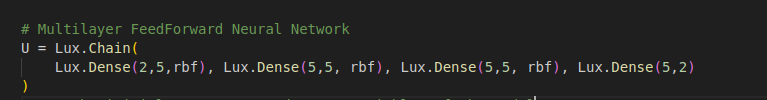
\includegraphics[width=0.45\textwidth]{plots/Screenshot from 2024-08-01 00-20-22.png}
    \caption{Network Initialization}
    \label{fig:network_initialization}
\end{figure}

The neural network was declared, using an RBF as the activation function in the dense layers. The network was then integrated into a Lotka-Volterra framework.

\begin{figure}[h]
    \centering
    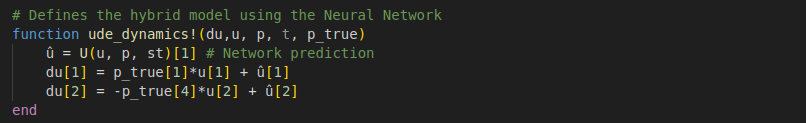
\includegraphics[width=0.45\textwidth]{plots/Screenshot from 2024-08-01 00-20-42.png}
    \caption{Integration into Differential Equation}
    \label{fig:integration}
\end{figure}

\section{Results and Discussion}
The results showed that the NODE model was effective in fitting and predicting trends from noisy Lotka-Volterra based training data. Figure \ref{fig:noisy_data} shows the noisy data generated from the Lotka-Volterra model used to train the neural network.

\begin{figure}[h]
    \centering
    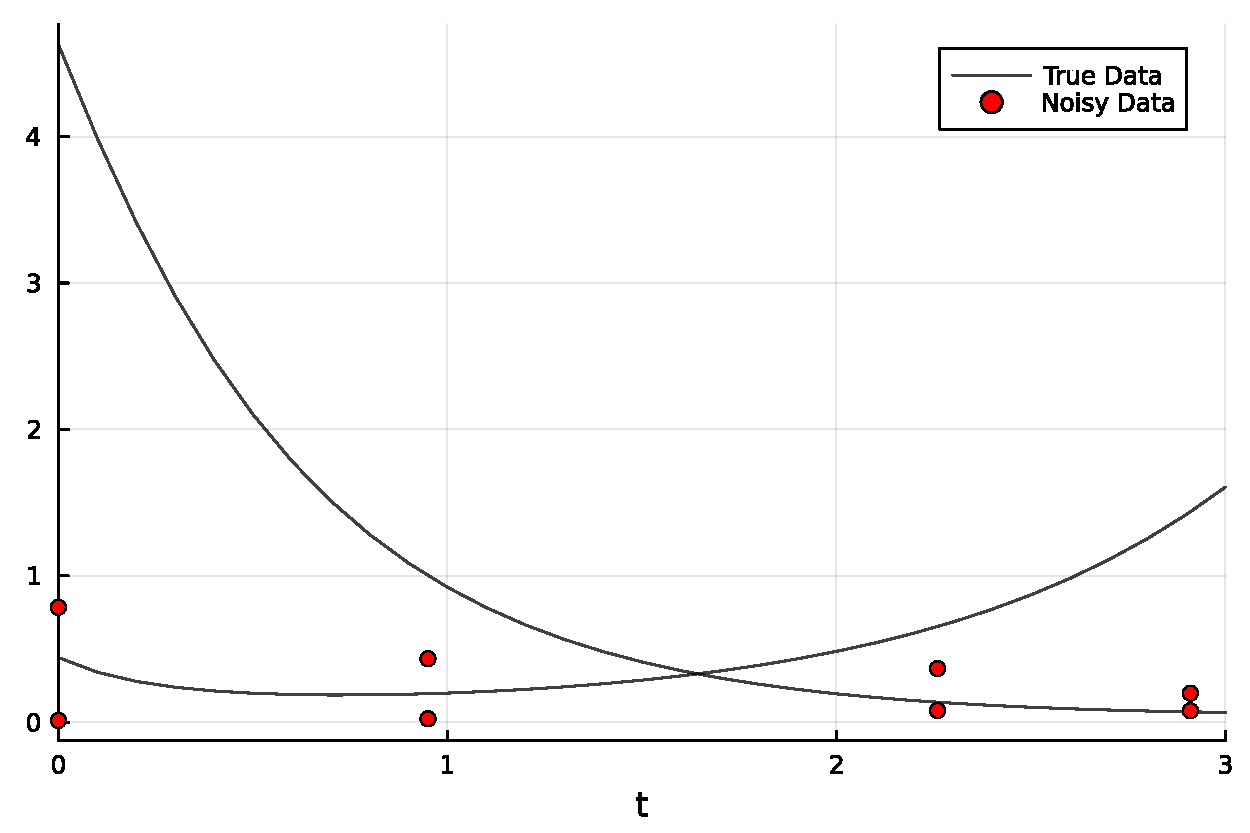
\includegraphics[width=0.45\textwidth]{plots/Chemostat_noisydata.pdf}
    \caption{Noisy Data}
    \label{fig:noisy_data}
\end{figure}

The training loss over iterations, shown in Figure \ref{fig:training_loss}, shows the performance of the NODE model during training. This shows that the ADAM optimizer did manage to reach a local minimum in the parameter space, and that once training with the activation function BFGS started, the loss decreased significantly further, indicating that BFGS was more effective at fine-tuning the parameters and finding a lower minimum. This demonstrates the advantage of using a combination of optimizers to achieve better training results.

\begin{figure}[h]
    \centering
    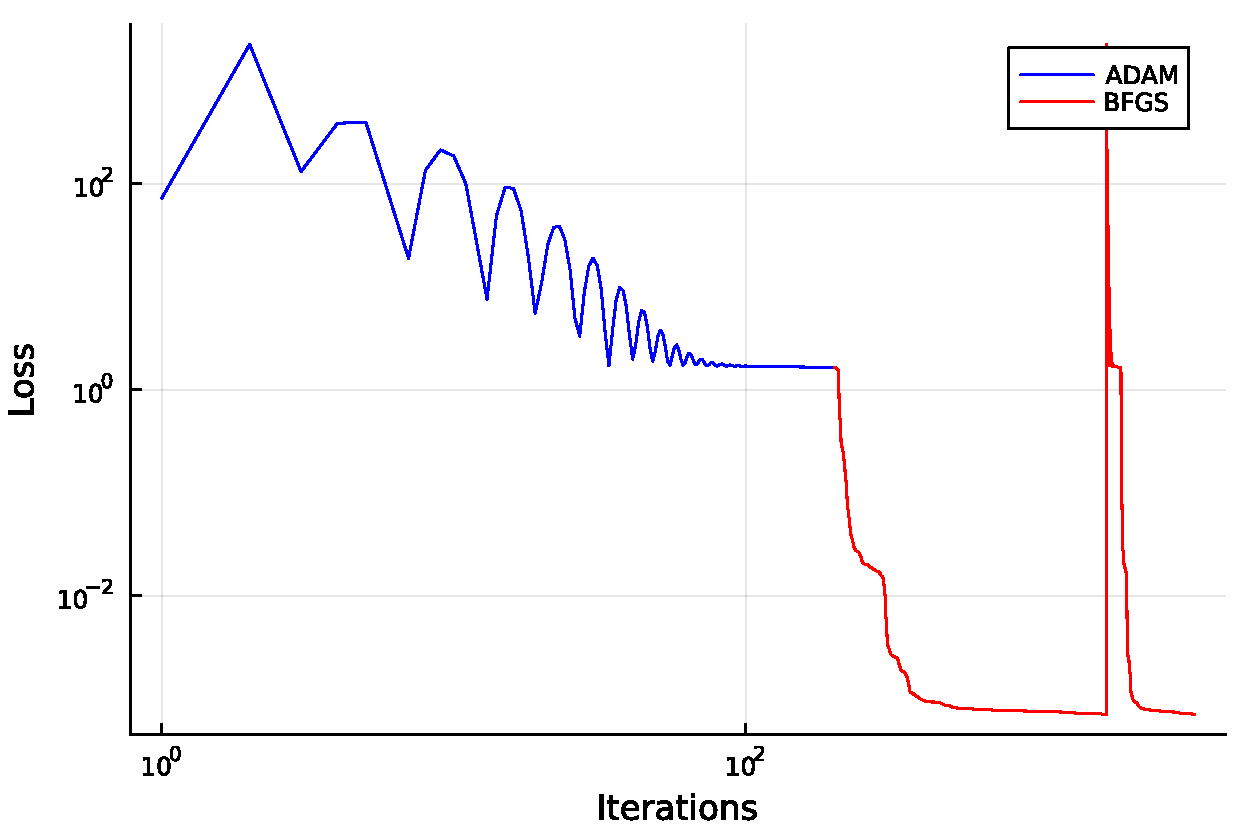
\includegraphics[width=0.45\textwidth]{plots/Ideal_Data__losses.pdf}
    \caption{Training Loss}
    \label{fig:training_loss}
\end{figure}

The trajectory reconstruction in Figure \ref{fig:trajectory_reconstruction} demonstrates the NODE model's ability to accurately learn the underlying prey and predator dynamics in noisy data, generated by the Lotka-Volterra curve.

\begin{figure}[h]
    \centering
    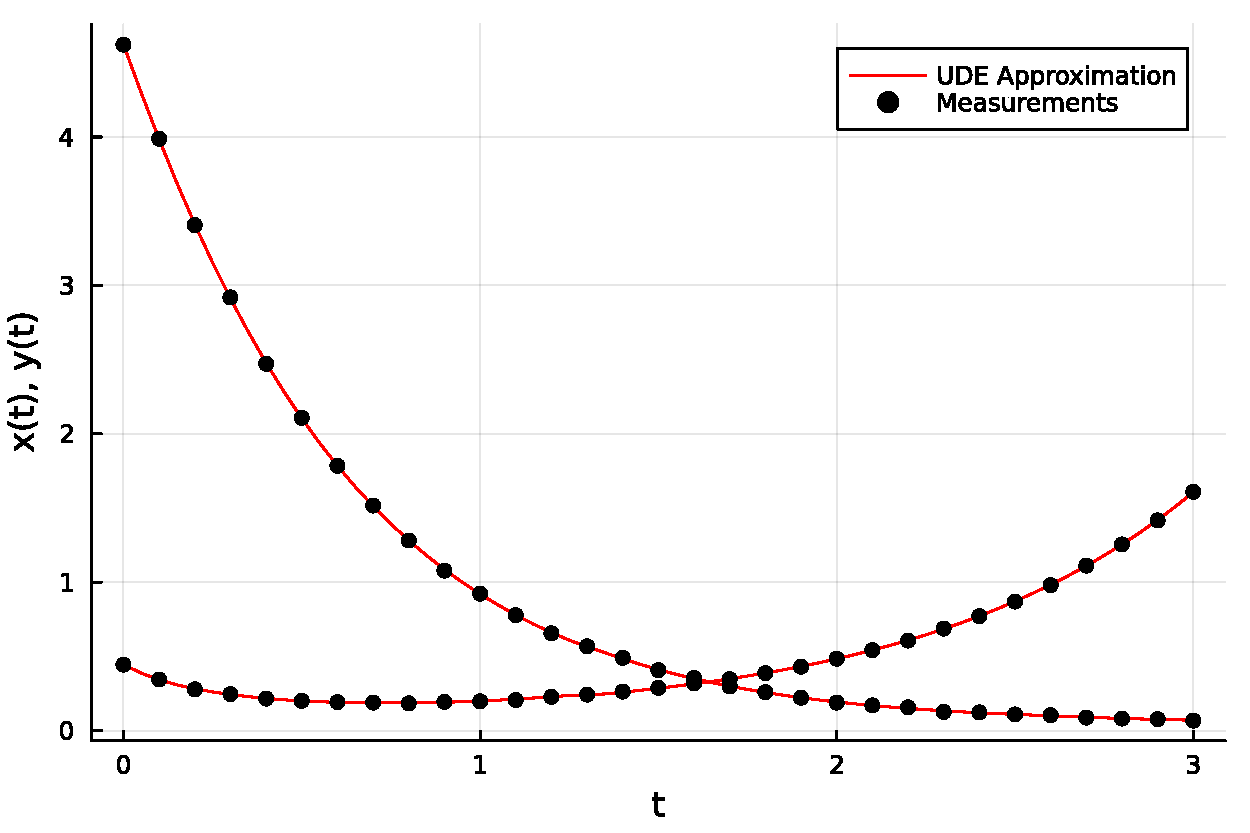
\includegraphics[width=0.45\textwidth]{plots/Ideal_Data__trajectory_reconstruction.pdf}
    \caption{Trajectory Reconstruction}
    \label{fig:trajectory_reconstruction}
\end{figure}

Figure \ref{fig:interaction_reconstruction} compares the neural network's approximation of the interaction terms to the true interaction terms in the Lotka-Volterra model. This demonstrates that, from the short training data, the neural network was able to accurately map the parameter space for both x and y values in the Lotka-Volterra system.

\begin{figure}[h]
    \centering
    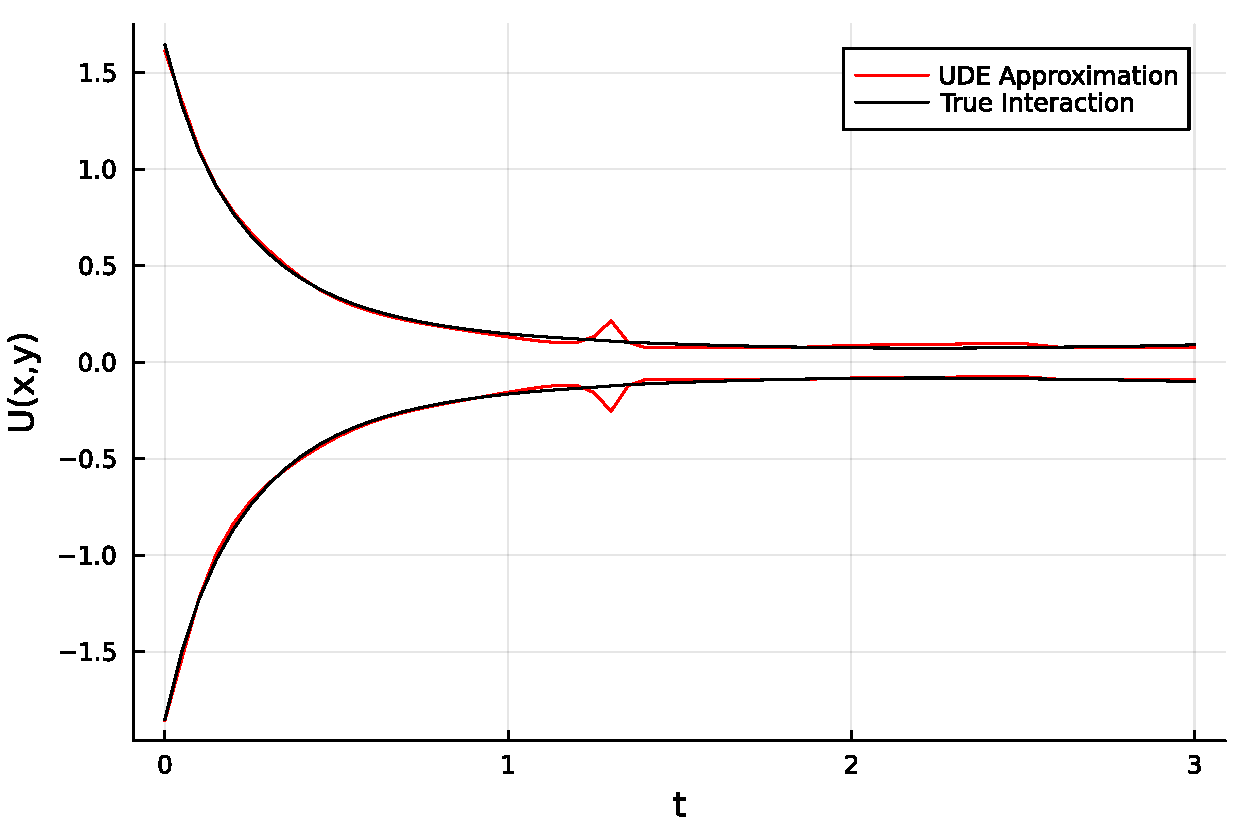
\includegraphics[width=0.45\textwidth]{plots/Ideal_Data__missingterm_reconstruction.pdf}
    \caption{Interaction Reconstruction}
    \label{fig:interaction_reconstruction}
\end{figure}

\FloatBarrier

The extended predictions of the classical Lotka-Volterra model over 50 time periods, shown in Figure \ref{fig:lotka_volterra_predictions}, highlight its oscillatory nature.

\begin{figure}[h]
    \centering
    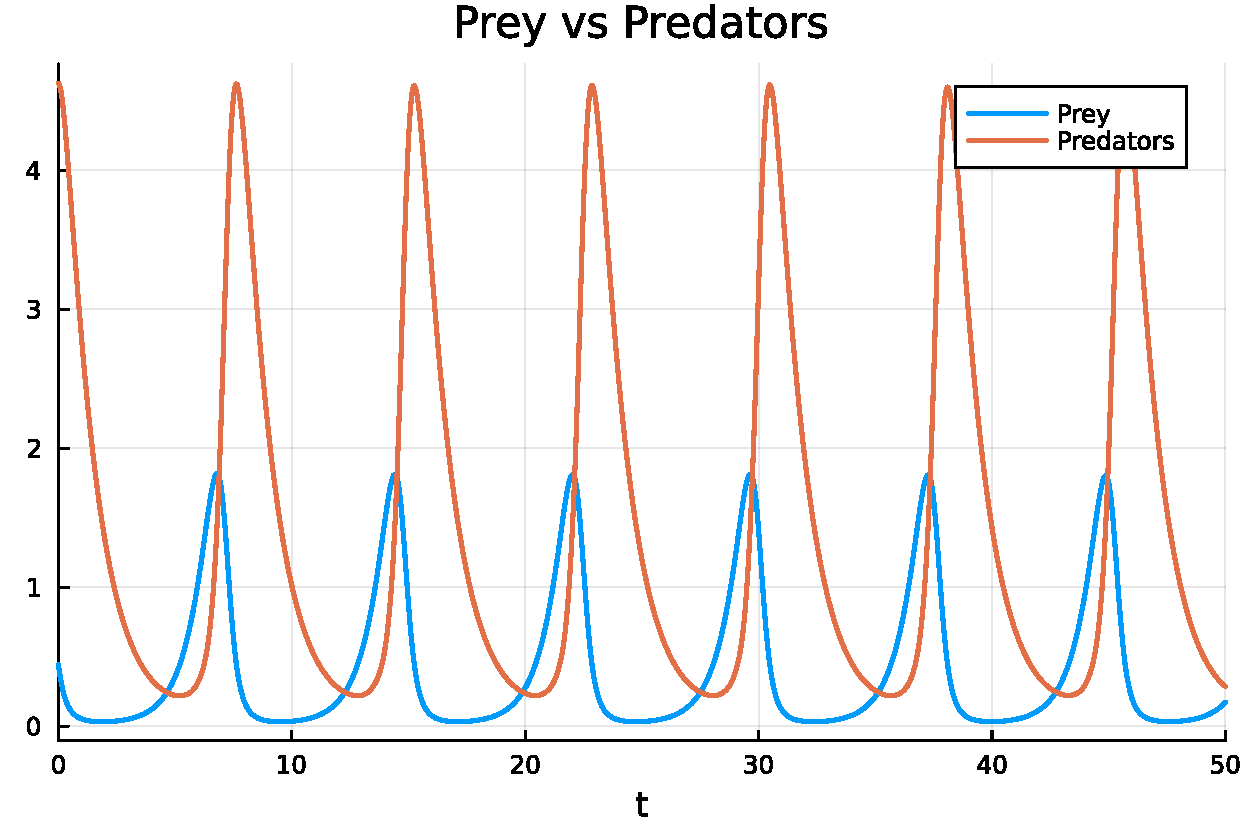
\includegraphics[width=0.45\textwidth]{plots/algae_vs_predators.pdf}
    \caption{Standard Lotka-Volterra Model}
    \label{fig:lotka_volterra_predictions}
\end{figure}

Figure \ref{fig:node_extrapolation} presents the NODE model's data extrapolation over 20 time periods, demonstrating its predictive capabilities beyond the training data.

\begin{figure}[h]
    \centering
    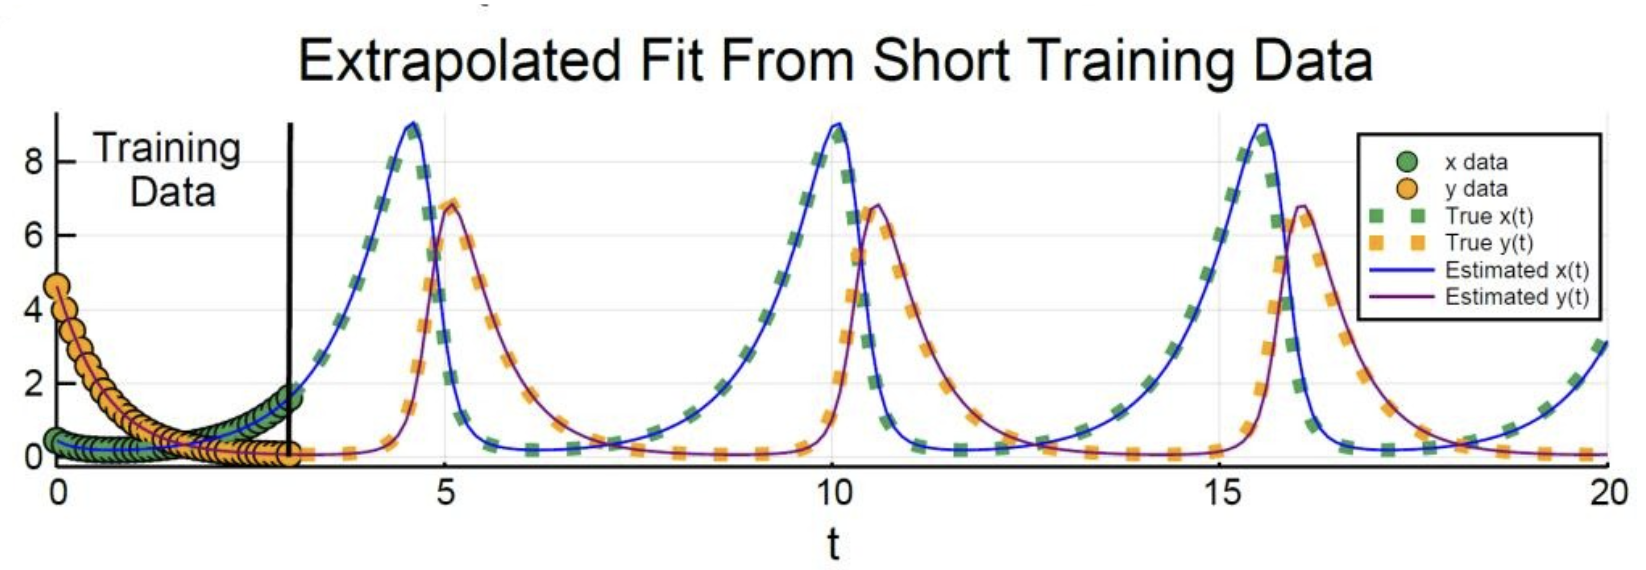
\includegraphics[width=0.45\textwidth]{plots/Extrapolated_fit.png}
    \caption{NODE Model Data Extrapolation}
    \label{fig:node_extrapolation}
\end{figure}

However, when applied to real experimental data of predator-prey interactions between Planktonic Rotifers and Unicellular Green Algae, the NODE model struggled to fit the data due to the high level of noise. Figures \ref{fig:real_data_application} and \ref{fig:real_data_loss} show the training data  and corresponding training losses, respectively.

\begin{figure}[h]
    \centering
    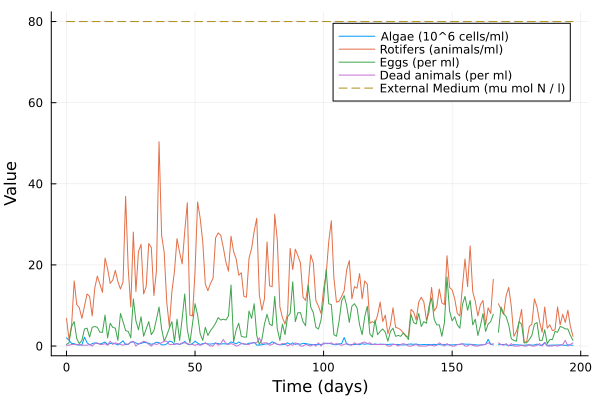
\includegraphics[width=0.45\textwidth]{plots/output_plot.png}
    \caption{Application to Real Data}
    \label{fig:real_data_application}
\end{figure}

\begin{figure}[h]
    \centering
    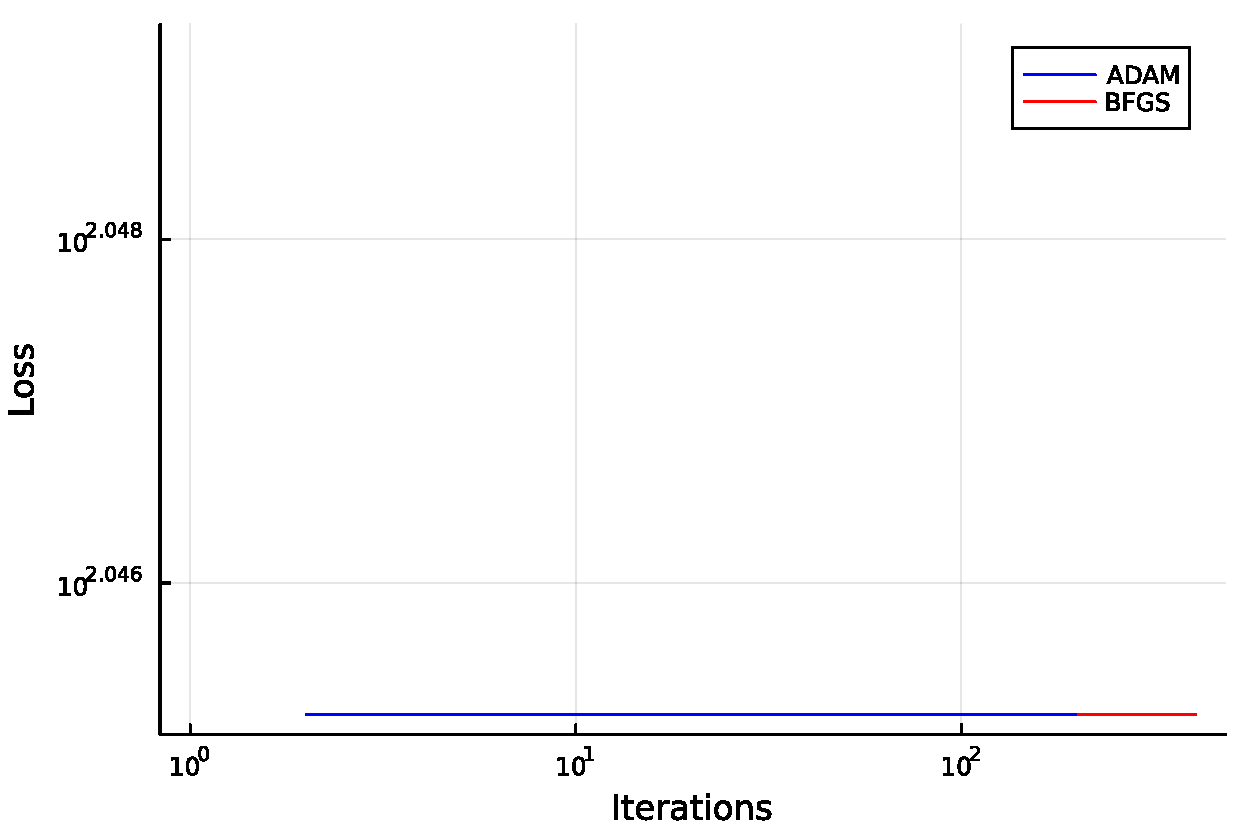
\includegraphics[width=0.45\textwidth]{plots/Chemostat_losses.pdf}
    \caption{Real Data Training Loss}
    \label{fig:real_data_loss}
\end{figure}

\FloatBarrier

These results show the NODE model's capability to capture trends in controlled synthetic environments but also its limitations when dealing with highly noisy real-world data.

\section{Future Implications}
The integration of larger neural networks and more sophisticated training algorithms could further enhance the accuracy and applicability of NODEs in ecological modeling. Future research could explore the application of NODEs to other ODE systems and biological interactions, potentially leading to a better understanding of complex ecological dynamics.

\section{Acknowledgements}
I would like to express my gratitude to my mentor Jeremey Van Cleve of the University of Kentucky for guiding me through this research project. I would also like to thank the Institute for Computing in Research for providing me with this opportunity.

-
\bibliographystyle{plain}
\bibliography{references}
\cite{Lotka1925}
\cite{Volterra1926}
\cite{Shertzer2014}
\cite{FIU_Lecture4}
\cite{Dunning1995}

\end{document}

